\documentclass[mode=present,paper=a4paper,orient=landscape, style=sailor]{powerdot}
\usepackage[czech]{babel}
\usepackage{times}
\usepackage[utf8]{inputenc}
\usepackage[T1]{fontenc}
\usepackage{amsmath}
\usepackage{amsthm}
\usepackage{amsfonts}
\usepackage{graphics}
\newcommand{\myuv}[1]{\quotedblbase#1\textquotedblleft}

\title{Úvod do tvorby prezentácií\\Typografia a~publikovanie}
\author{Patrik Holop}
\date{2017}

\begin{document}
\maketitle

\begin{slide}{Motivácia}
\begin{itemize}
\item \textbf{Prečo sa nimi zaoberať?}\\
	-- Zaujatie publika\\
	-- Udržanie pozornosti\\
	-- Ukážky grafov a~obrázkov\\
	-- Pohodlná tvorba\\
	-- $\cdots$\\
\end{itemize}
\begin{itemize}
\item \textbf{Kde môžeme prezentácie využiť?}\\
	-- Školské prostredie\\
	-- Prezentácia produktov\\
	-- Zasadania a~stretnutia\\
	-- Vyhodnotenie výsledkov\\
	-- $\cdots$\\
\end{itemize}
\end{slide}

\begin{slide}{Dôležité kroky}
\begin{itemize}
\item \textbf{Načo nezabudnúť}\\
	-- Úvodný slide a~predstavenie\\
	-- Slidy by mali obsahovať:\\
	\hspace{1.5em}  -- Nadpis, text, odrážky\\
	\hspace{1.5em}  -- Obrázky, grafy\\
	\hspace{1.5em}	-- Iné prvky (citácie ad.)\\			  	  
	-- Použité zdroje\\
	-- Poďakovanie za pozornosť\\
	-- $\cdots$\\
\end{itemize}
\begin{quotation}
\textit{\bfseries \myuv{Dobrá prezentácia je podobná zaujímavej knihe. Ak ju vytvoríte správne, poslucháč bude s~radosťou čakať na ďalší slide.}}
\end{quotation}
\end{slide}

\begin{slide}{Správne vyjadrovanie}
\begin{itemize}
\item \textbf{Prezentácia slúži len ako podpora!}
\item \textbf{Dôležitý je prejav a~vyjadrovanie}\\
		-- Nehovorte monotónne a~nezaujato\\
		-- Poslucháč musí vidieť vaše zaujatie\\ 
\item Oživenie prezentácie humorom
\end{itemize}
\begin{itemize}
\item \textbf{Ďalšie rady}\\
	    -- pohľad do publika\\
	    -- rečnícke prestávky\\
	    -- nesnažte sa rýchlo ukončiť prezentáciu\\
\end{itemize}
\begin{quotation}
\textit{\bfseries \myuv{Aký je človek sám, taká je aj jeho reč.}\\ \hspace{12em}Cicero}
\end{quotation}
\end{slide}

\begin{slide}{Časté chyby}
\begin{itemize}
\item \textbf{Dizajn a~slidy}\\
        -- Bežné šablóny z~editorov\\
        -- Ponechanie základného fontu\\
        -- Veľa efektov a~textu\\
        -- Všetko na slidoch\\
\vspace{1em}
\item \textbf{Rečník}\\
        -- Všetko číta\\
        -- Málo vlastného prínosu\\
\end{itemize}
\begin{quotation}
\textit{\bfseries \myuv{Nehovorte o~chybách, tie budú hovoriť samy za seba.}\\ \hspace{12em}Winston Churchill}
\end{quotation}
\end{slide}

\begin{slide}{Príklad správneho slidu}
\begin{itemize}
\item Krátke výstižné odrážky\\
	-- Popisom ich môžeme rozviť\\
\item Nie je ich príliš veľa\\
\item Dôležité pojmy môžeme \textbf{zvýrazniť}\\
\item Na zaujatie sme použili obrázok
	-- Musí súvisieť s~obsahom slidu
\end{itemize}
\vspace{-1em}
\begin{figure}[h]
\scalebox{0.33}{
\includegraphics{publikum.eps}}
\caption[Obrázok]{Zaujaté publikum\footnote{\tiny http://www.personal-erfolg.de/ihr-publikum-entscheidet-was-eine-gute-praesentation-ist/}}
\end{figure}
\end{slide}

\begin{slide}{Príklad nesprávneho slidu}
\begin{itemize}
\item Nepodstatná odrážka obsahujúca veľa textu, ktorý poslucháča odradí si ju prečítať. Všetok text má jednotný štýl a~nie je rozdelený do odrážok. Všimnite si obrázok nižšie a~jeho popis. Nielenže je vidieť nízku kvalitu, ale ani vôbec nesúvisí s~témou. 
\begin{figure}[h]
\scalebox{0.50}{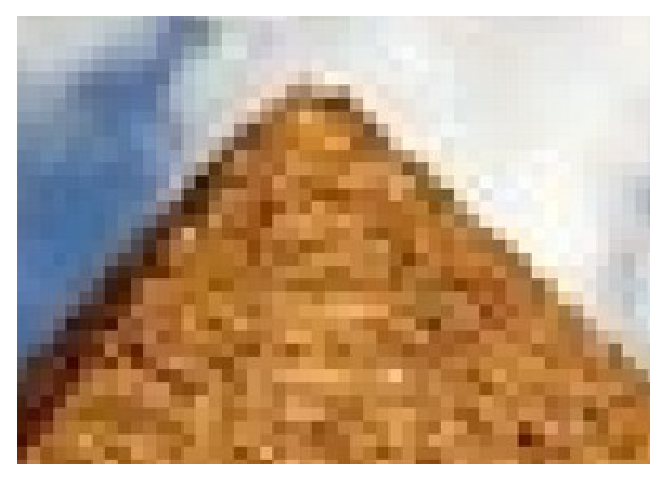
\includegraphics{pyramida.eps}}
\caption[Obrázok] {Obrázok má nízku kvalitu a~nesúvisí s~témou\footnote{http://infika.wz.cz/uvod-do-grafiky.html}}
\end{figure}
\end{itemize}
\end{slide}


\begin{slide}{Použité zdroje}
\begin{itemize}
\item BENNÁR, Peter. \textit{5 najčastejších chýb pri tvorbe POWERPOINT prezentácie} [online, cit. 29.4.2017]. Dostupné z: http://pekneprezky.sk/5-najcastejsich-chyb-pri-tvorbe-prezentacie-v-powerpointe/
\item Citácie\\ http://citaty-slavnych.sk/
\end{itemize}
\end{slide}

\end{document}